% Define document class
\documentclass[twocolumn]{aastex631}
\usepackage{amssymb}
%\documentclass[modern]{aastex631}

% Some entries inspired from a preamble by Adrian Price-Whelan, https://github.com/adrn/PhaseSpiralAsteroseismology/blob/main/tex/preamble.tex

\usepackage{showyourwork}

% Latex imports
\let\tablenum\relax             % necessary for AASTeX
\usepackage{siunitx}
\sisetup{range-phrase=-, range-units=single, separate-uncertainty=true}
\sisetup{separate-uncertainty=true}
\usepackage{blindtext}          % Filler text
\usepackage{xcolor}

% paper comments
\usepackage{comment}						 % comments that can be switched visible/invisible
\includecomment{comment}
%\specialcomment{outtake}{\begingroup\sffamily\color{gray}}{\endgroup}
\specialcomment{note}{\begingroup\sffamily\color{red!40!green!70!blue!90}}{\endgroup}
%\excludecomment{note}                       % switch notes off

%% switch TODO notes on/off
\usepackage[backgroundcolor=red!20!green!40!blue!10, textsize=tiny]{todonotes}
\usepackage{regexpatch}
\makeatletter
\xpatchcmd{\@todo}{\setkeys{todonotes}{#1}}{\setkeys{todonotes}{inline,#1}}{}{}
\makeatother
%\usepackage[disable]{todonotes}			% switches all todo notes to invisible

% ---------------------------------
% PAPER VARIABLES
\newcommand{\Nplanets}{\ensuremath{733}}
\newcommand{\percentageTransiting}{999}
\newcommand{\dmax}{\ensuremath{50\,\mathrm{pc}}}
\newcommand{\wrr}{0.001}
\newcommand{\windowsize}{25}
\newcommand{\prSmin}{10}
\newcommand{\prSmax}{1000}
\newcommand{\prWRRmin}{10^{-5}}
\newcommand{\prWRRmax}{0.1}
\newcommand{\prRmin}{0.1}
\newcommand{\prRmax}{15}


% ---------------------------------
% CONSTANTS/MISSIONS/ABBREVIATIONS

% SIunitx definitions
\DeclareSIUnit\mSun{M_\odot}
\DeclareSIUnit\Msun{M_\odot}
\DeclareSIUnit\mStar{M_\star}
\DeclareSIUnit\Mstar{M_\star}
\DeclareSIUnit\mEarth{M_\oplus}
\DeclareSIUnit\Mearth{M_\oplus}
\DeclareSIUnit\rEarth{R_\oplus}
\DeclareSIUnit\Rearth{R_\oplus}
\DeclareSIUnit\year{yr}
\DeclareSIUnit\au{au}
\DeclareSIUnit\dex{dex}
\DeclareSIUnit\ppm{ppm}
\DeclareSIUnit\eV{eV}

% Missions/Projects/Packages
\newcommand{\project}[1]{\textsl{#1}}
\newcommand{\rst}{\project{Nancy Grace Roman Space Telescope}}
\newcommand{\plato}{\project{PLATO}}
\newcommand{\cheops}{\project{CHEOPS}}
\newcommand{\kepler}{\project{Kepler}}
\newcommand{\emcee}{\project{emcee}}

% Stats / probability
\newcommand{\given}{\,|\,}
\newcommand{\norm}{\mathcal{N}}
\newcommand{\pdf}{\textsl{pdf}}

% Maths
\newcommand{\dd}{\mathrm{d}}
\newcommand{\transpose}[1]{{#1}^{\mathsf{T}}}
\newcommand{\inverse}[1]{{#1}^{-1}}
\newcommand{\argmin}{\operatornamewithlimits{argmin}}
\newcommand{\mean}[1]{\left< #1 \right>}

% Non-scalar variables
\renewcommand{\vec}[1]{\ensuremath{\bs{#1}}}
\newcommand{\mat}[1]{\ensuremath{\mathbf{#1}}}

% Unit shortcuts
\newcommand{\msun}{\ensuremath{\mathrm{M}_\odot}}
\newcommand{\mjup}{\ensuremath{\mathrm{M}_{\mathrm{J}}}}
\newcommand{\kms}{\ensuremath{\mathrm{km}~\mathrm{s}^{-1}}}
\newcommand{\mps}{\ensuremath{\mathrm{m}~\mathrm{s}^{-1}}}
\newcommand{\pc}{\ensuremath{\mathrm{pc}}}
\newcommand{\kpc}{\ensuremath{\mathrm{kpc}}}
\newcommand{\kmskpc}{\ensuremath{\mathrm{km}~\mathrm{s}^{-1}~\mathrm{kpc}^{-1}}}
\newcommand{\dayd}{\ensuremath{\mathrm{d}}}
\newcommand{\yr}{\ensuremath{\mathrm{yr}}}
\newcommand{\AU}{\ensuremath{\mathrm{AU}}}
\newcommand{\Kel}{\ensuremath{\mathrm{K}}}

% Misc.
\newcommand{\bs}[1]{\boldsymbol{#1}}

% Astronomy
\newcommand{\feh}{\ensuremath{{[{\rm Fe}/{\rm H}]}}}
\newcommand{\mh}{\ensuremath{{[{\rm M}/{\rm H}]}}}
\newcommand{\logg}{\ensuremath{\log g}}
\newcommand{\Teff}{\ensuremath{T_{\textrm{eff}}}}
\newcommand{\vsini}{\ensuremath{v\,\sin i}}
\newcommand{\gaia}{\textsl{Gaia}}

% Begin!
\begin{document}

% Title
\title{The imprint of global magma oceans on exoplanet demographics}

% Author list
\author[0000-0001-8355-2107]{Martin Schlecker}
\affiliation{Department of Astronomy/Steward Observatory, The University of Arizona, 933 North Cherry Avenue, Tucson, AZ 85721, USA}
\author{al.}


% Abstract
\begin{abstract}
    $\ldots$ magma oceans $\ldots$

    Here, we assess the ability of space and ground-based telescopes to test this hypothesis using Bioverse, a simulation framework that leverages contextual information from the overall planet population.
    $\ldots$

%    We argue that in the near future, ESA's \plato\ mission and NASA's Roman Space Telescope will be the most promising endeavors to constrain this demographic feature.
%    For each of these missions, we identify the key mission design drivers that enable a statistically sound detection.
%    We also show the unique synergy of these missions in answering this question, and what survey strategy optimizes the statistical power of the combined dataset.
%    $\ldots$ its measurement will also provide insights into which stars harbor the nearest habitable worlds.
\end{abstract}

% Main body
\section{Introduction}
...just dropping material and references for now...
\todo[inline]{papers: \citep[][introduce runaway GH]{} \citep[][statistical detection of GH transition]{Turbet2019}, \citep[][water loss, O2 buildup around M dwarfs]{Luger2015}, \citep[][Solubility of H in magma oceans]{Hirschmann2012,SchlichtingShahar_inreview,} \citet{Hamano2013,Hamano2015,Barth2021,Downey2022}.}



\begin{note}
For observations of rocky exoplanets, the currently best-probed regime is that of warm, close-in planets.
These bodies experience climatic conditions that are similar to the environment of the inner Solar System bodies at early stages of their formation.
Studies of the geophysical state and evolution of hot exoplanets can thus contribute to our understanding of the early formation stages of Earth and other habitable worlds.

...
    Venus and Earth, while having accreted from the same mass reservoir and despite their similar bulk properties, evolved into planets with very different environmental conditions on their surfaces.
    At the formation of the Solar System, both planets underwent a giant impact phase [CITE!] that melted their mantles, leading to a magma ocean stage.
    Due to these similar early formation phases, it was commonly assumed that the divergence of Venus and Earth -- in particular Venus's water loss -- occurred late in their evolution~\citep{Elkins-Tanton2013}.
    \citet{Hamano2013} showed that such a late desiccation process is not needed to explain the stark differences: for a planet rich in volatiles and receiving high enough radiation levels from its host star, a steam atmosphere limits the outgoing radiation from the (molten) planetary surface.
    This runaway greenhouse state prevents the planet's rapid cooling and can extend the magma ocean stage to hundreds of \SI{}{\mega\year}, enough to remove the entire water reservoir from a rocky planet by hydrodynamic escape.
    \todo[inline]{important for motivating the existence of the pattern: ``the solidification timescale can become comparable to the main-sequence lifetime of the star (Hamano et al. 2013, 2015)'' \citep{Lichtenberg2022} }
    Under the right conditions, different orbital distances alone can thus decide about a planet's water content and ultimately its habitability.
    If received flux makes the difference between our own habitable planet and dry, dead Venus, there is good reason to believe that such patterns exist in exoplanet systems as well.

    ...long-term goal/overarching objective: derive the geophysical history of rocky extrasolar planets. More concrete: Constrain the limits of runaway greenhouse transitions, and thus the inner edges of the habitable zone. Also: How close is Earth from this runaway greenhouse irradiation limit?
   ...
\todo[inline]{introduce magma oceans and their influence on planetary radii~\citep{Dorn2021}.}
    ...current/future observations of planets that are currently in the runaway greenhouse phase may constrain properties of their planetary mantles... make connection between interior and atmospheres.
    ...
    Planetary radius changes due to the combined effect of steam atmospheres and water dissolved in the molten mantle of planets within the runaway greenhouse threshold is expected to cause a discontinuity in the radius distribution of small (DEFINITION) exoplanets.
\end{note}


\section{Methods}\label{sec:methods}
\todo[inline]{Caveats: see \citet{Turbet2019} Sect. 3, \citet{Bower2019}}
%The purpose of this paper is to demonstrate the feasibility of measuring the demographic feature introduced above with near-future exoplanet missions.

We determined -- for different survey configurations -- the confidence level with which the runaway greenhouse threshold can be detected in simulated exoplanet observations.
For this purpose we expanded the Bioverse framework~\citep{Bixel2020,Bixel2021}\footnote{Bioverse is actively maintained and documented open source software written in Python. Its latest version and documentation can be found at \url{https://github.com/danielapai/bioverse}.} to generate synthetic stellar and planetary samples into which we injected the runaway greenhouse signal, simulated observations of this sample, and computed Bayesian evidences in favor of the runaway greenhouse hypothesis (see diagram in Fig.~\ref{fig:flowchart}).
\begin{figure*}
    \begin{centering}
        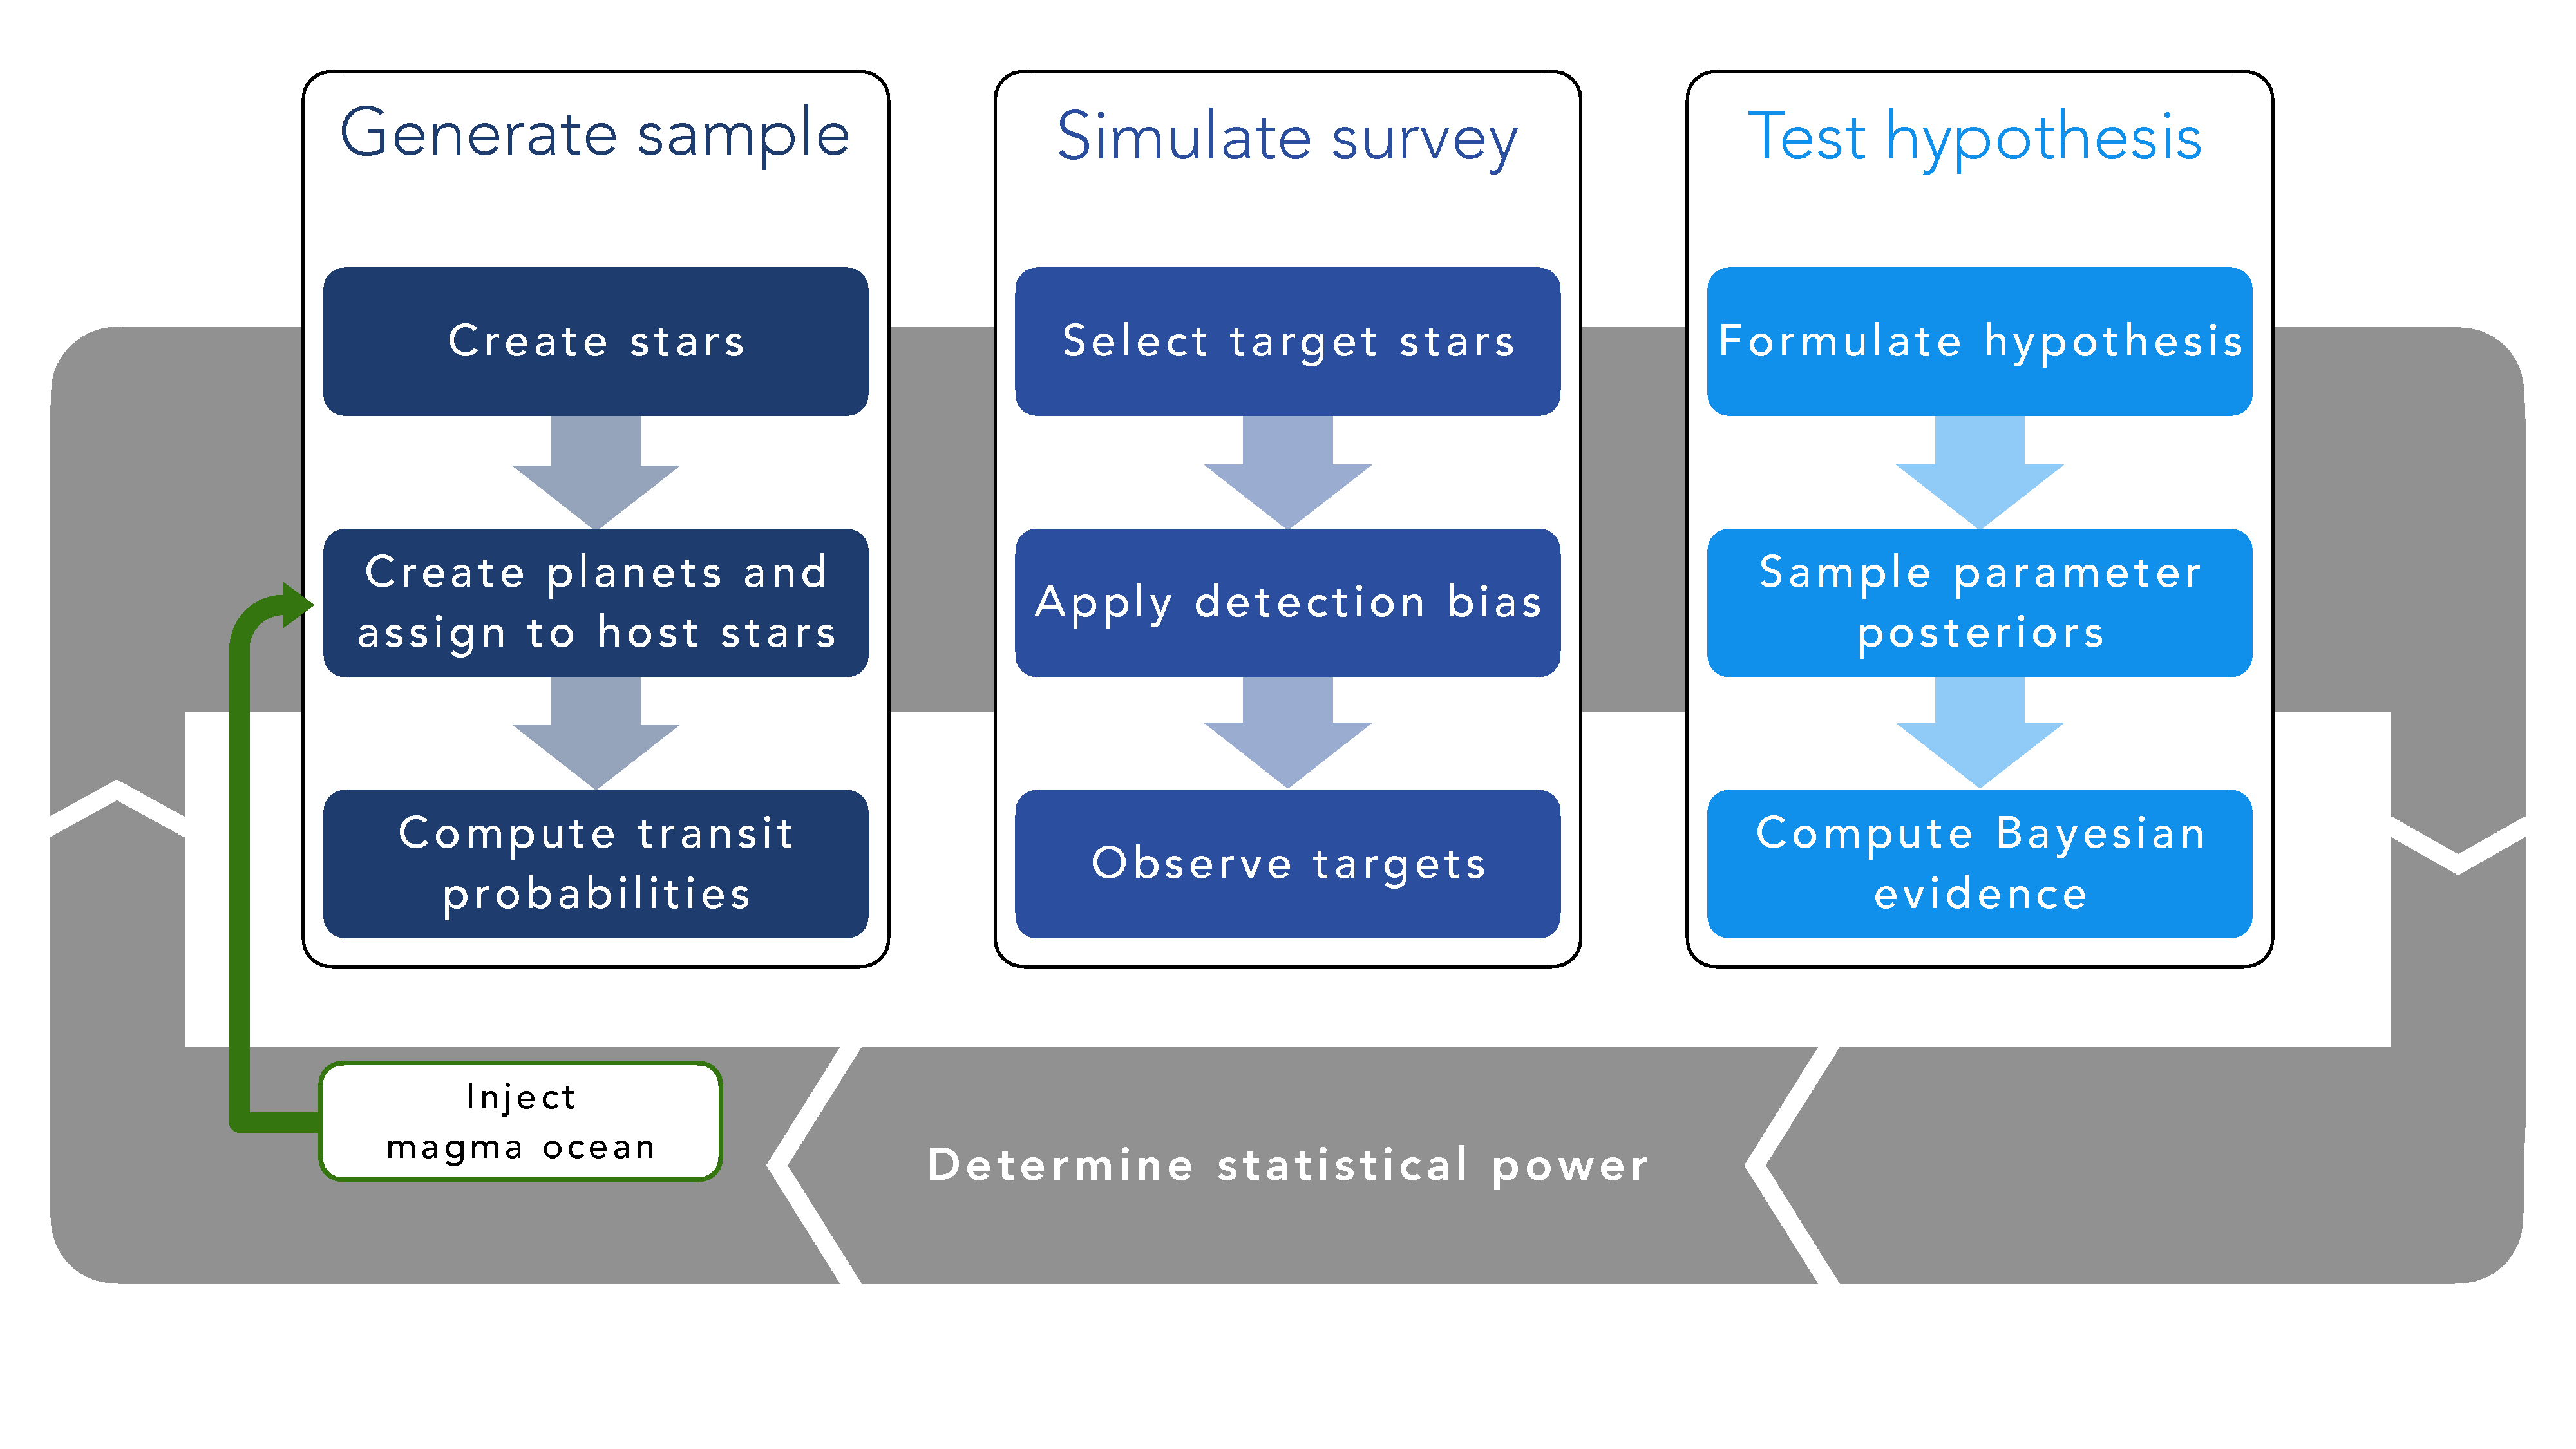
\includegraphics[width=\hsize]{figures/flowchart.pdf}
        \caption{Workflow of our hypothesis testing with Bioverse. In the first block, we generate a sample of stars and populate them with planets based on \kepler\ demographics.
            A fraction of them are then assigned a runaway greenhouse climate based on the model described in Sect.~\ref{sec:mo_model}.
        The second block simulates an exoplanet survey, whereby selection effects and detection biases are introduced. Finally, the third block deals with testing the runaway greenhouse hypothesis based on data from the survey simulation.
        By iterating through these steps, we compute the statistical power of testing the hypothesis given the assumed survey design.}
        \label{fig:flowchart}
    \end{centering}
\end{figure*}



\subsection{Synthetic star and planet sample}
The first step in our analysis is to generate a sample of stars that host synthetic planets.

\subsubsection{Stellar sample from Gaia DR3}
Different sample sizes are realized by varying the maximum distance of stars to the solar system $d_\mathrm{max}$.
\todo[inline]{KEVIN: describe stellar population}
...

\subsubsection{Stellar luminosity tracks}
    Planetary systems are hosted by stars of a wide range of ages, and stellar luminosities evolve with time.
    Since the emergence of a runaway greenhouse phase on a planet is highly dependent on the level of radiation it receives, and thus on the luminosity of the host star, we assigned age-dependent luminosities to our synthetic stars.
    Stellar ages are notoriously poor-constrained (CITE); we thus drew random ages from a uniform distribution from \SI{0}{\giga\year} to \SI{10}{\giga\year}.
    We then assigned each star a luminosity from the mass-dependent evolutionary models in \citet{Baraffe1998}.
    Figure~\ref{fig:luminosity_tracks} shows the corresponding luminosity evolution as a function of stellar mass and age.
\begin{figure}[ht!]
    \script{plot_luminosity_tracks.py}
    \begin{centering}
        \includegraphics[width=\linewidth]{figures/luminosity_tracks.pdf}
        \caption{
            Bolometric luminosity tracks of stars with different masses, computed from stellar evolution models in \citet{Baraffe1998}.
            Low-mass stars, which make up the majority of stars in the solar neighborhood, undergo an extended early phase of several magnitudes higher luminosity before entering a lifetime of relative faintness.
        }
        \label{fig:luminosity_tracks}
    \end{centering}
\end{figure}


\subsubsection{Synthetic planet sample}\label{sec:syn_planets}
Next, we assigned to the stellar sample planetary systems with frequencies, orbital parameters, and bulk properties derived from the \kepler\ mission.
We adopted the planetary occurrence rates in orbital period and radius recently derived in~\citep{Bergsten2022}.
Following \citep{Youdin2011a}, their inferred occurrence rate density can be expressed in the form
\begin{equation}
    \frac{\mathrm{d}^2n}{\mathrm{d}R \, \partial P} = F_0 C_n g(R, P),
\end{equation}
where $F_0$
...
\todo[inline]{GALEN: Briefly describe underlying planet occurrence rates of synthetic population, its Mstar dependency, any caveats or assumptions.}


\subsubsection{Eccentricities, orbital inclinations, and planet masses}
Eccentric orbits alter the probability of a planet to transit \citep[e.g.,][]{Barnes2007a}.
The distribution of eccentricities $e$ of exoplanets has been found to resemble a Beta function \citep{Kipping2013b}, which we chose to draw synthetic eccentricities from.
Following~\citet{Kipping2013b}, we used a Beta distribution with parameters $a=0.867$ and $b=3.03$, and truncated the distribution at $e = 0.8$.

Another parameter with an even higher impact on transit probabilities is the orbital inclination toward the observer $i$.
Assuming isotropic alignments of orbits, we assigned each planet an inclination drawn from a distribution uniform in $\cos(i)$.

To assign masses to our planets, we use the semi-empirical mass-radius relationship derived in \citet{Zeng2016}.
The default relation our planets follow is one assuming a pure $\mathrm{MgSiO_3}$ composition.
\todo[inline]{JUSTIFY this choice (TIM?)}
\todo[inline]{run a test: do we expect that the choice of M-R relation impacts the results? Perhaps have an appendix section.}
This represents the baseline bulk density before any climate-related effects are applied.


\subsubsection{Transit probability}
\begin{note}
    We model the occurrence of transits by assuming isotropic orientations of planetary orbits, calculating the impact parameters $b = \cos(i)/R_\star$ and considering only observable planets with $|b| < 1$.
    For these cases we calculate the transit depth
    \begin{equation}\label{eq:transitdepth}
        \delta = \left( \frac{R_\mathrm{P}}{R_\star} \right)^2,
    \end{equation}
    which is relevant for the detection probability of the respective planet~(see Sect.~\ref{sec:sensitivity}).
    Excluding all non-transiting planets diminishes the sample to \SI{\percentageTransiting}{\percent} of its original size.
\end{note}


\subsubsection{Planet radius changes due to runaway greenhouse climates}\label{sec:mo_model}
\todo[inline]{"Methods Section" for the geophysical models. Describe specific parametrization, dependency on bulk planet/orbit params\\
~\\
\textbf{Main assumptions:}\\
- Assume that every planet has \textit{some} water. Enough for runaway GH under the right conditions. Baseline water content: 20\% \\
- Limitation to small planets without significant atmospheric envelopes.\\
- we ignore water loss by H$_2$O photolysis in the upper atmosphere and subsequent H escape, which would eventually cool even planets within the runaway greenhouse regime~\citep{Lichtenberg2022}.\\
- we ignore tidal heating, which could extend the magma ocean phase of close-in planets (and change their orbits via tidal orbital evolution)( Jackson et al., 2008; Barnes et al., 2013 (?)).\\
}
...


\todo[inline]{ARNAUD: revise definition of $S$ following our discussion on 2022-12-22. Introduce net instellation and clarify what is meant by it.}
\begin{note}
    The power from the host star per unit area at the position of a planet or instellation $S$ in units of Earth's insolation is given by
    \begin{equation}
        \frac{S}{S_\oplus} = \left(\frac{L_\star}{L_\odot}\right) \left(\frac{au}{a}\right)^2 .
    \end{equation}
    Here, we assume global redistribution of incoming flux and a fixed albedo of $0.3$, comparable to Earth's [CITE].
    The absolute value of $S_\oplus$, by which all synthetic planets are scaled, is then \SI{238}{\watt\per\square\meter}.
%    We further define the solar-equivalent semi-major axis $a_{eff} = a (L_\star/L_\odot)^{-1/2}$, at which a planet experiences the same instellation as a Solar System planet at an orbital distance~$a$.
\end{note}







    Central to our procedure is to explore the detectability of population-level trends with future exoplanet surveys, and here the trend in question is the proposed radius discontinuity.
    To enable a quantitative assessment of this detectability, we injected the signal into the simulated planet sample before observing it with simulated surveys.
    While we search for the runaway greenhouse pattern in demographic quantities such as average planet radii, the injected changes happen on the planetary level: We changed each planet's radius based on its individual set of properties and the associated predictions from steam atmosphere and water incorporation models.
    Relevant properties are a planet's mass $M$, its instellation $S$, and its bulk water inventory expressed as a water mass fraction $x_{H_2O}$.
    We consider three different cases:
    \begin{itemize}
   \item[A.] No radius change.
    This case serves as our null hypothesis, where planetary radii are not affected by the amount of irradiation the planets receive.
    A solid planetary surface is assumed and no steam atmosphere is present.
   \item[B.] Radius inflation due to a steam atmosphere.
    Atmospheric scale heights are significantly increased.
   \item[C.] As B, but including radius decrease of inflated planets due to water partitioning in the molten mantle.
    \end{itemize}


In case~A, a planet simply retains the radius it was assigned based on exoplanet occurrence rates (see Sect.~\ref{sec:syn_planets}).
There is no additional dependency on orbital distance or instellation.

Case~B assumes an inflated radius due to a steam atmosphere for all planets receiving a dayside-averaged instellation exceeding a threshold of $S_\mathrm{thresh} = \SI{280}{\watt\per\meter\squared}$.
This value was found to be a limit for the flux a planet can emit in a runaway greenhouse situation~\citep{Goldblatt2013,Leconte2013}.
To quantify the radius change, we applied the mass-radius relationships derived by \citet{Turbet2020} using a 1D~inverse radiative-convective model~\citep{Turbet2019}.
For the rocky interiors, their calculations rely on the same mass-radius relations from ~\citep{Zeng2016} that we applied for case~A-planets.
For each planet above the instellation threshold, we assigned the predicted radius for the given water mass fraction and planet mass.
We note that an additional radius change due to potentially molten interiors~\citep{Bower2019} is not taken into account here.

Case~C contains case~B, but also includes a radius decrease due to water partitioning in the melt.
Due to greenhouse forcing, planetary surfaces below steam atmospheres are expected to be molten.
Part of the water will then partition into the melt, removing it from the steam atmosphere, which in turn decreases the radius inflation.
This effect is generally small compared to the radius inflation from a steam atmosphere but resulting radius changes typically reach measurable values~\citep{Dorn2021}.
The magnitude of this effect is again dependent on the planet mass and on the water mass fraction.
We follow \citet{Dorn2021} and use their computed radius deviations between a wet magma ocean and a solid mantle for a tropopause pressure~$P_\mathrm{iso}=\SI{0.1}{\bar}$.
We then add the (in almost all cases negative) radius deviations to the planet radii computed for case~B.

\begin{figure}
    \begin{centering}
        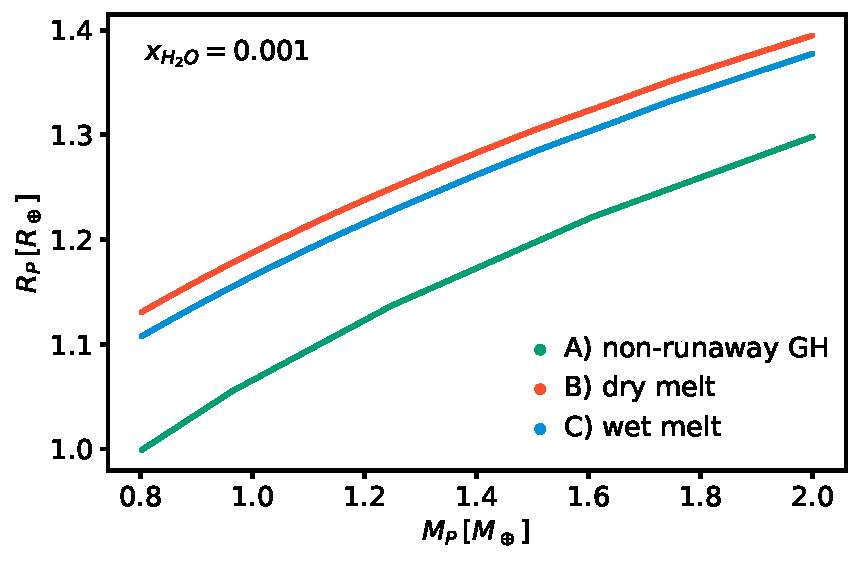
\includegraphics[width=\hsize]{figures/radiuscomparison.pdf}
    \end{centering}
    \begin{centering}
        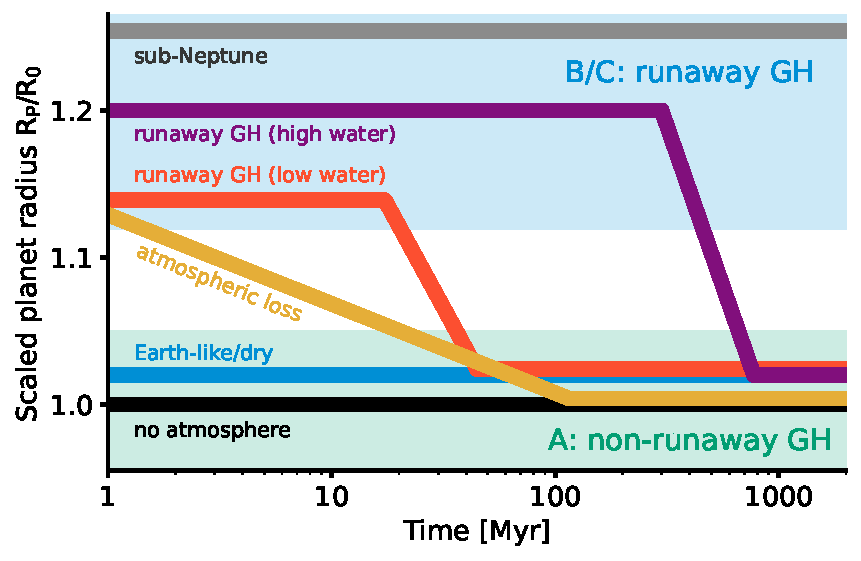
\includegraphics[width=\hsize]{figures/radiusevolution.pdf}
        \caption{
            \textit{Top}: Mass-radius relationships for a water mass fraction $x_{H_2O}= \wrr$ and different planet states: A) planets with a solid mantle and no steam atmosphere. B) planets with steam atmospheres. C) as B), but including the effect of water incorporation in the melt.
            \textit{Bottom}: Radius evolution of different planet types, illustrating degeneracies among planet classes. Shown is a schematic time evolution of the transit radius normalized to the atmosphere-free radius $R_\mathrm{0}$ for different scenarios. Planets can move between planet classes through processes such as atmospheric loss and desiccation, which ultimately ends a runaway greenhouse phase on a timescale dependent on a planet's water content.}
        \label{fig:radiusevolution}
    \end{centering}
\end{figure}
Figure~\ref{fig:radiusevolution} shows the different mass-radius relations of the three cases for a fiducial water mass fraction of $x_{H_2O}= \wrr$.
Steam atmospheres (case~B) cause a significant radius increase, which is slightly reduced when water incorporation in the melt is allowed (case~C).
In the following, we only distinguish between cases~A and~C.

As illustrated in Fig.~\ref{fig:radiusevolution}~(bottom panel), different processes can lead to the classification of a planet into either of these categories.
For instance, both a Hydrogen/Helium-dominated ``sub-Neptune'' and a terrestrial planet currently hosting a steam atmosphere will appear as a case~C planet, diluting the expected demographic signature.
Further, a planet in a runaway greenhouse state will eventually lose its steam atmosphere and move to category~A~\citep[e.g.,][]{Hamano2013}.
To account for these effects, we introduce a free parameter $f_\mathrm{rgh}$ representing the fraction of planets above the threshold instellation that are currently inflated due to a runaway greenhouse climate.
Our simulation setup is such that all planets receiving an instellation $S < S_\mathrm{thresh}$ follow relation~A, and a fraction $f_\mathrm{rgh}$ of the planets with $S > S_\mathrm{thresh}$ follow relation~C.
%The choice $f_\mathrm{rgh} < 1$ comprises all reasons why a planet has no runaway greenhouse climate despite high instellation, for instance the absence of an atmosphere or of volatiles that could form a steam atmosphere, or prior complete desiccation.
This parametrization introduces a discontinuity of average planet radii and bulk densities as a function of stellar irradiation.
In the following, we test if and under what conditions this trend is large enough to be detected with high significance.




\subsection{Survey simulations}
The survey module of Bioverse converts the synthetic planet sample into a set of uncertainty-laden measurements on a subset of that sample.
   This task includes selection of the targets, application of detection biases, and conducting simulated measurements.
   All of the above are specific to the particular survey.

\subsubsection{Detection bias and sample selection}\label{sec:sensitivity} % Turbet2019 lists precision for CHEOPS, PLATO?, TESS?
Not all transiting planets are detectable with the same likelihood and detection biases have an impact on the demographic measurements we are interested in.
A detailed characterization of the detection biases of individual missions would not be justifiable given the uncertainties of the theoretical predictions.
Instead, we derived generic observing limits that reflect the limitations of state-of-the-art transit surveys.

The runaway greenhouse transition is expected to occur at orbits sufficiently close to let mission duration not be a limiting factor: $S_\mathrm{thresh}$ occurs close to Earth's orbital period for \mbox{G-type} stars and on significantly shorter periods for the more prevalent M~dwarf hosts~\citep{Goldblatt2012}.
However, for a transit signal to be detected in a transit survey, it must reach a sufficient signal-to-noise ratio (S/N).
This S/N is sensitive on the photometric precision that can be achieved~\citep[e.g.,][]{Burke2015,Hardegree-Ullman2019}.
In its in-orbit commissioning phase, the \cheops\ mission demonstrated a photometric precision of \SI{75}{\ppm} for faint ($V\approx 12$) stars~\citep{Benz2021}.
In comparison, \plato's expected precision for similar stars was estimated to be \SI{\sim 50}{\ppm}~\citep[][Matuszewski et al., in prep.]{plato2017}.
To represent these photometric limits, we chose a minimum transit depth of \SI{75}{\ppm} as a detection limit and consider only measurements of planets exceeding this threshold.
We further exclude target stars with \gaia\ magnitudes $M_\mathrm{G} > \minMagnitude$.

%    Current and near-future missions focusing on Earth-sized planets target several host star spectral types, and their exact sample selection is based on specific mission objectives.
%    We thus chose a broad selection function centered on general detectability of transits with state-of-the-art technology.
The runaway greenhouse effect becomes obsolete where no atmosphere can be maintained due to proximity to the host star and resulting atmospheric erosion.
We thus excluded planets with extremely high instellation that does not allow long-term preservation of an atmosphere and clear our sample from all planets with an instellation $S > \SI{2000}{\watt\per\square\meter}$.
\todo[inline]{use criterion of Zahnle \& Caitling 2017 instead? $0.8 S^{0.25} < R$}
We further consider only rocky planets with masses below \SI{2}{\Mearth}. % (Turbet+2020 covers only 0.1 to 2 Mearth)


\subsection{Hypothesis tests}
We now turn to assessing the simulated surveys in terms of their ability to detect the runaway greenhouse transition and their constraining power on parameters of this trend.
To do this, we rely on a Bayesian hypothesis testing approach where we quantify the evidence of a hypothesis over another based on the (simulated) data.
For our specific problem, this implies comparing evidences for a demographic imprint of the runaway greenhouse effect to its absence.
\subsubsection{Definition of the runaway greenhouse hypothesis}
\begin{note}
%    Bayesian model comparison requires that an alternative mode be specified against which the comparison is made.
\end{note}
    As a null hypothesis, we consider the case where the planetary radius distribution is independent of the instellation,
    \begin{equation}
        H_0(\theta, S) = \theta,
    \end{equation}
    where $\theta$ is the set of parameters defining the radius distribution.
    We further define an alternative hypothesis that describes radius changes due to steam atmospheres and water in the melt.
    As motivated above, this hypothesis takes the form of a step function in instellation $S$, where the step occurs at the outer edge of the runaway greenhouse region.
    Our main observable shall be the average planet radius in the planet population inside and outside this threshold.
    The runaway greenhouse hypothesis is then defined as
\begin{equation}\label{eq:rgh_hypo}
    H_{\mathrm{rgh}}(\theta, S) =
        \begin{cases}
            H_0, &  S \leq S_\mathrm{thresh}\\
            \langle R_\mathrm{P}\rangle (f_\mathrm{rgh},\Delta R_\mathrm{stm}, \Delta R_\mathrm{wtr}), &  S > S_\mathrm{thresh}.
        \end{cases}
\end{equation}
    Here, $f_\mathrm{rgh}$ is the fraction of planets experiencing a runaway greenhouse effect.
    $\Delta R_\mathrm{stm}$ and $\Delta R_\mathrm{wtr}$ are predicted radius changes from the steam atmosphere and water incorporation models, respectively.
    They are assumed to act additively on the planet radii and thus on their average $\langle R_\mathrm{P}\rangle $.

The only free parameter of the null hypothesis, which assumes the average radius to be independent of instellation, is the predicted mean radius $\langle R_\mathrm{P}\rangle $.
The functional form of the runaway greenhouse hypothesis is more complex: Besides the mean radius of planets outside the threshold $\langle R_\mathrm{P}\rangle_\mathrm{out}$, which is a nuisance parameter necessary to define the hypothesis, it relies on the threshold instellation for the ``step'' $S_\mathrm{thresh}$, the planetary water mass fraction~$x_{H_2O}$ encoding the amount of radius change, and the fraction of planets above the threshold instellation that are in a runaway greenhouse climate $f_\mathrm{rgh}$.

The measured radii $R_\mathrm{P, i}$ cannot be directly used for the hypothesis tests as they include intrinsic scatter that is not caused by measurement errors.
$H_{\mathrm{rgh}}$ and $H_0$ should thus be tested against a statistical estimator that represents the population mean.
To avoid binning and the artificial patterns it may introduce, we chose to test our hypotheses against a simple moving average $SMA$ along the instellation axis with a window of size \windowsize\ centered around each measurement.
We further computed the uncertainty of this moving average by propagating the individual measurement errors and applying a rolling standard error of the mean. \todo[inline]{specify error propagation}

As our procedure involves random sampling of the model parameters $\theta$, we need to define the probability of obtaining a dataset given the model parameters, i.e., a likelihood function.
We assumed here that the individual moving averages $SMA_i$ are measured with a normally distributed uncertainty $\sigma_{SMA_i}$ and adopted a normal distribution
\begin{equation}
    \mathcal{L}(SMA \mid \boldsymbol{\theta})=\prod_{i}^{N} \frac{1}{\sqrt{2 \pi \sigma_{SMA_i}^{2}}} \exp \left(-\frac{\left(SMA_i - H\left(\boldsymbol{\theta}, S_i\right)\right)^{2}}{2 \sigma_{SMA_i}^{2}}\right).
\end{equation}
Here, $H\left(\boldsymbol{\theta}, S_i\right)$ corresponds to the functional form of the runaway greenhouse or null hypothesis.



\subsubsection{Bayesian model comparison}
We are now ready to assess the relative plausibility of $H_{\mathrm{rgh}}$ and $H_0$ given the synthetic data we have generated, assigning equal a~priori~ probabilities to these models.
This is done by comparing the Bayesian evidence $\mathcal{Z}$ of the models, which we estimate with the nested sampling~\citep{Skilling2004} algorithm \emph{dynesty}~\citep{Speagle2020}.
Our criterion to reject the null hypothesis is
\begin{equation}
\Delta \ln \mathcal{Z}  = \ln \mathcal{Z}_\mathrm{rgh} - \ln \mathcal{Z}_0  > 3.
\end{equation}
The chosen threshold roughly corresponds to the $p = 0.05$ threshold for statistical significance popular in frequentist approaches.\todo{CITATION}

A sensible choice of priors is central for evidence estimation via nested sampling.
As the parameters we are interested in recovering, $S_\mathrm{thresh}$ and $x_{H_2O}$, are poorly constrained by previous data, we used relatively uninformative priors to sample the entire physically plausible parameter space.
For $S_\mathrm{thresh}$, we chose a log-uniform prior in $[\prSmin,\prSmax]\, \SI{}{\watt\per\meter\squared}$.
Similarly, we sample $x_{H_2O}$ from a log-uniform distribution to imply scale-invariant ignorance.
Its boundaries $[\prWRRmin, \prWRRmax]$ are motivated by the water mass fractions covered by the geophysical models~(Sect.~\ref{sec:mo_model}).
Finally, we adopt a broad, uniform prior for $\langle R_\mathrm{P}\rangle_\mathrm{out}$ bound by $[\prRmin, \prRmax] \, \mathrm{R_\oplus}$.
We then ran the nested sampler to compute the evidence and sample the posterior distributions.



\section{Results}
\subsection{Statistical signature of the runaway greenhouse threshold}
To characterize the population-level imprint of individual radius changes, we generated a generic planet population with an injected runaway greenhouse effect assuming a water fraction $x_\mathrm{H_2O} = \wrr$.
\begin{figure}
    \begin{centering}
        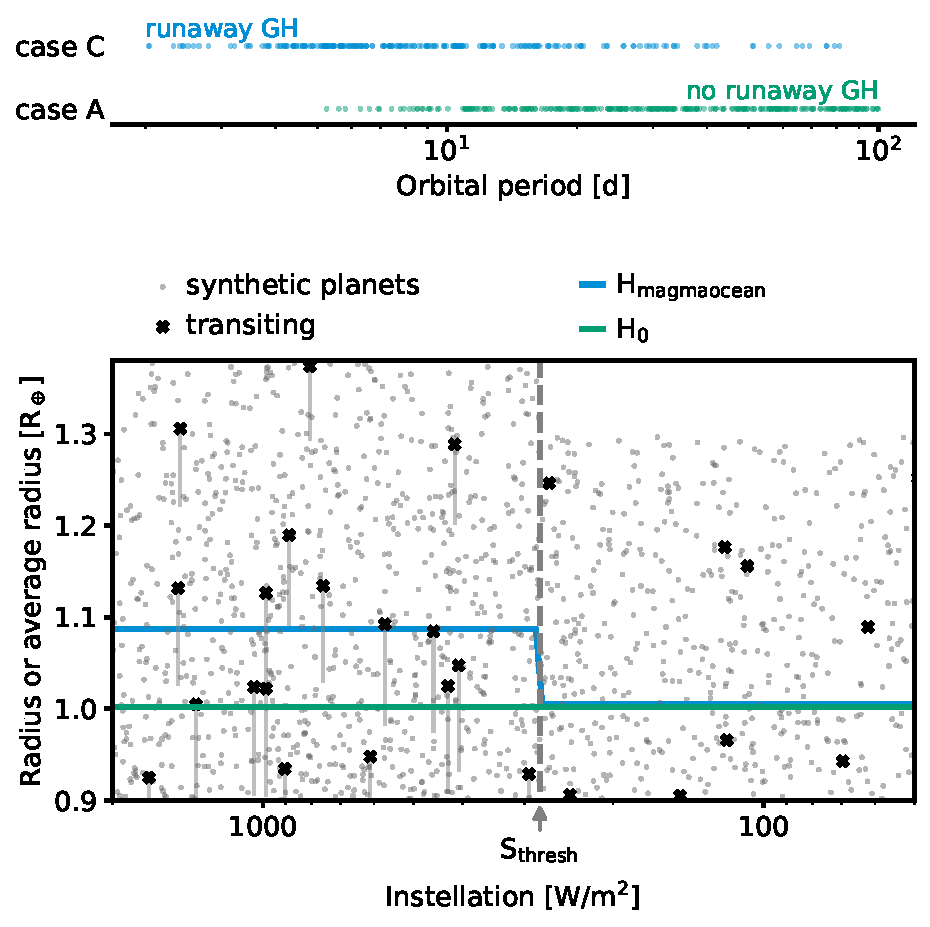
\includegraphics[width=\hsize]{figures/HnullHmo.pdf}
        \caption{Synthetic planets above and below the runaway greenhouse threshold.
        \textit{Top}: Planet state as a function of orbital period. Planets with and without a runaway greenhouse climate mix and are not distinguishable in period space.
        \textit{Bottom}: Radii of synthetic planets with injected radius deviation as a function of instellation. Only the planets marked as transiting are observable. Above the runaway greenhouse threshold $S_\mathrm{thresh} =\SI{280}{\watt\per\meter\squared} $, the radii of a fraction of planets are inflated by the amount indicated with gray lines. The sharp boundary at $S_\mathrm{thresh}$ causes a discontinuity in the average planet radius (blue). This runaway greenhouse hypothesis can be tested against the null hypothesis $H_0$ (green), where average radii are independent of instellation.}
        \label{fig:HnullHmo}
    \end{centering}
\end{figure}
Figure~\ref{fig:HnullHmo} shows the resulting planetary radii.
When ordered in orbital period space, the different planet types overlap, diluting the demographic imprint.
With net instellation as an independent variable, planets above and below the runaway greenhouse threshold separate.
We also show the predictions of observable average planet radii from the statistical hypotheses defined above.
%The value for the average radius \textit{outside} the runaway greenhouse regime was computed from our nominal observed sample, whereas the radius change in the magma ocean case compared to the null hypothesis is a prediction from the magma ocean model, evaluated on the same sample.
Within the runaway greenhouse limit, an average radius change of \avgRadiusChange\ occurs.


\subsection{Testability of the runaway greenhouse hypothesis}
\begin{figure}[ht!]
%    \script{figurescript.py}
    \begin{centering}
        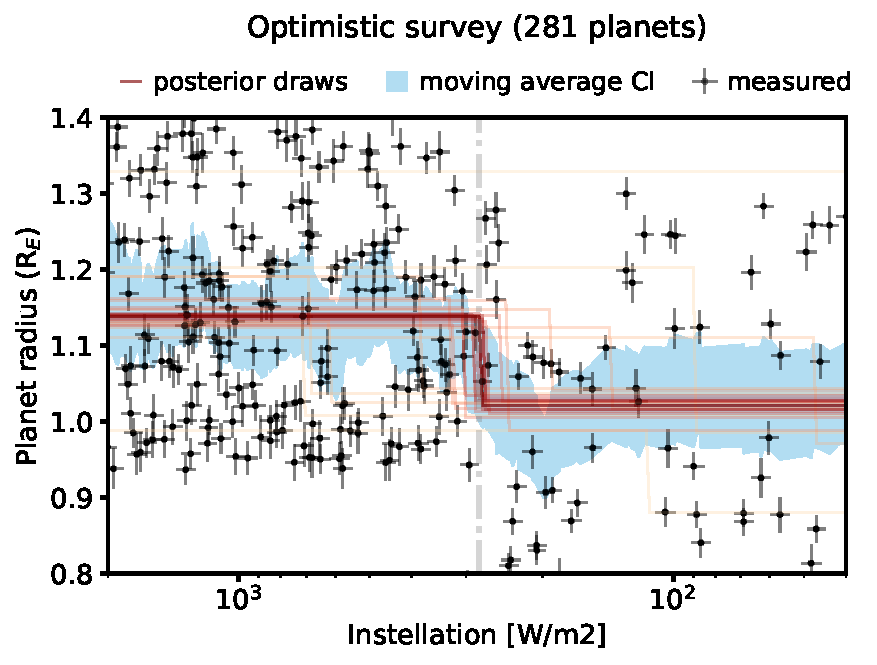
\includegraphics[width=\linewidth]{figures/optimistic_R-S.pdf}
        \caption{
        Detection of the runaway greenhouse threshold in the optimistic case.
        From simulated radius and instellation measurements of a large ($N = \var{N_optimistic}$) survey, we compute the moving average (blue confidence intervals) and fit the runaway greenhouse hypothesis to it (Eqn.~\ref{eq:rgh_hypo}, random draws from the posterior in red).
            The pattern is detected with high significance.
        }
        \label{fig:optimistic_R-S}
    \end{centering}
\end{figure}
Figure~\ref{fig:optimistic_R-S} shows a prototypical detection of the runaway greenhouse threshold.
For the sake of clarity, we chose an optimistic scenario where the sample is large ($N = \var{N_optimistic}$) and the measurement uncertainties are small ($\sigma_{R} = \sigmaR, \sigma_{S} = \sigmaS$).
We assumed that the fraction of those planets irradiated stronger than $S_\mathrm{thresh}$ that have runaway greenhouse climates is \frgh, and we chose a water mass fraction of \wrr\ for each planet.
In this case, the pattern was detected with high significance ($\Delta \ln \mathcal{Z} \approx 100$).


\begin{figure}[ht!]
%    \script{figurescript.py}
    \begin{centering}
        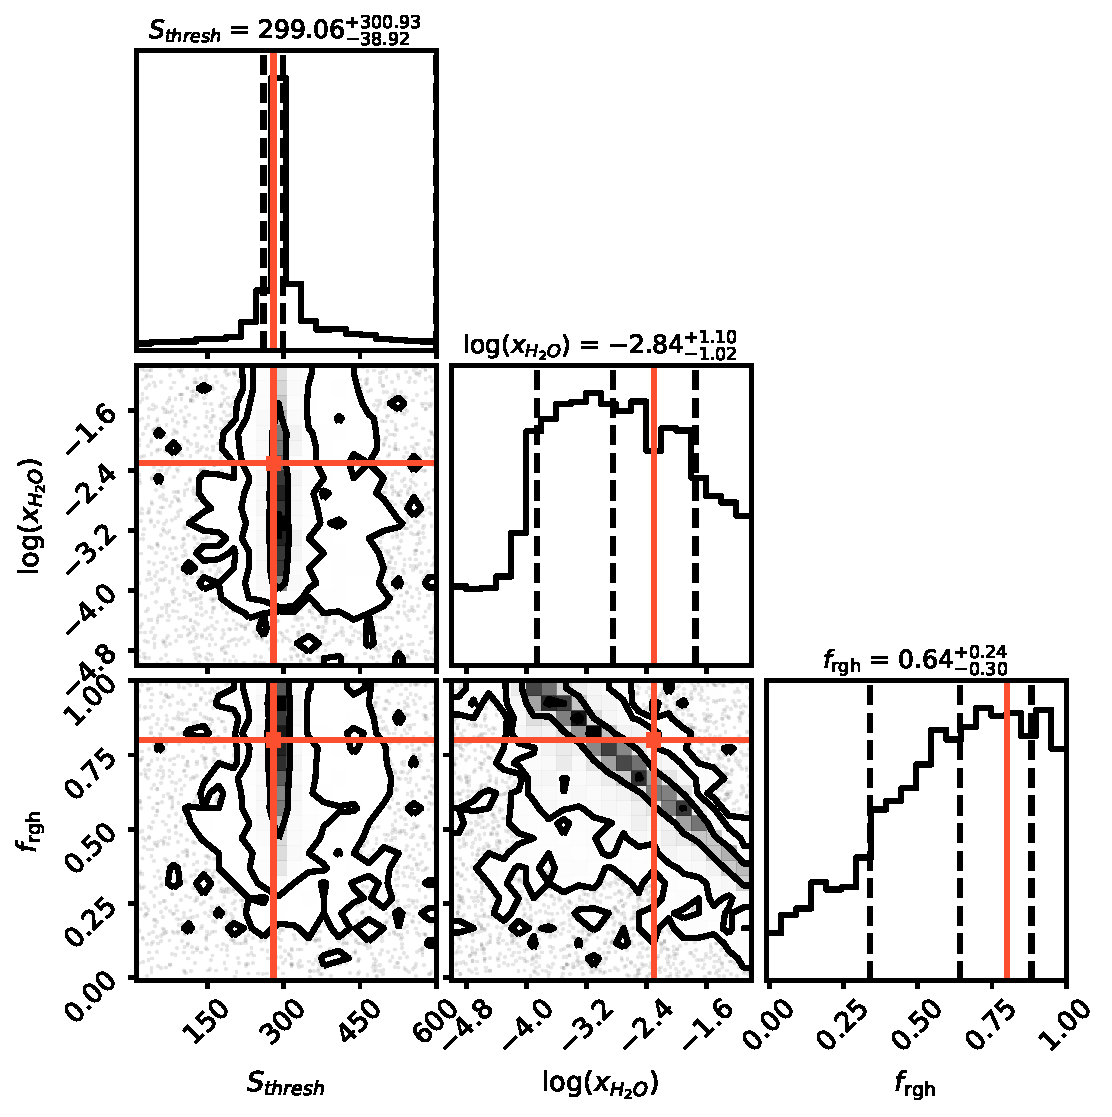
\includegraphics[width=\linewidth]{figures/corner.pdf}
        \caption{
            Retrieved posterior distribution of key parameters in the optimistic scenario. The density maps in each panel show relationships between and marginalized distributions of the model parameters as they could be retrieved with a high-precision transit survey and a sample of \var{N_optimistic} planets. True values of the parameters for the injected effect are shown in orange. The threshold instellation can be well constrained; the predominant water fraction and the fraction of planets with runaway greenhouse climates are degenerate.
        }
        \label{fig:cornerplot}
    \end{centering}
\end{figure}
With such a strong signal, we can attempt an inference of the parameters defining the injected effect.
Figure~\ref{fig:cornerplot} shows the posterior distributions of $S_\mathrm{thresh}$, $x_{H_2O}$, and $f_\mathrm{rgh}$ as determined by the nested sampler.
The threshold instellation can be accurately constrained with a median $\hat{S}_\mathrm{thresh} = \var{retrSthresh}$.
Both a higher water mass fraction and a higher fraction of planets in a runaway greenhouse state lead to larger average radii, thus these parameters are strongly correlated and cannot be well constrained without independent measurements.

Given an optimistic survey design, what influences the probability of correctly rejecting a false null hypothesis?
\begin{figure}[ht!]
%    \script{figurescript.py}
    \begin{centering}
        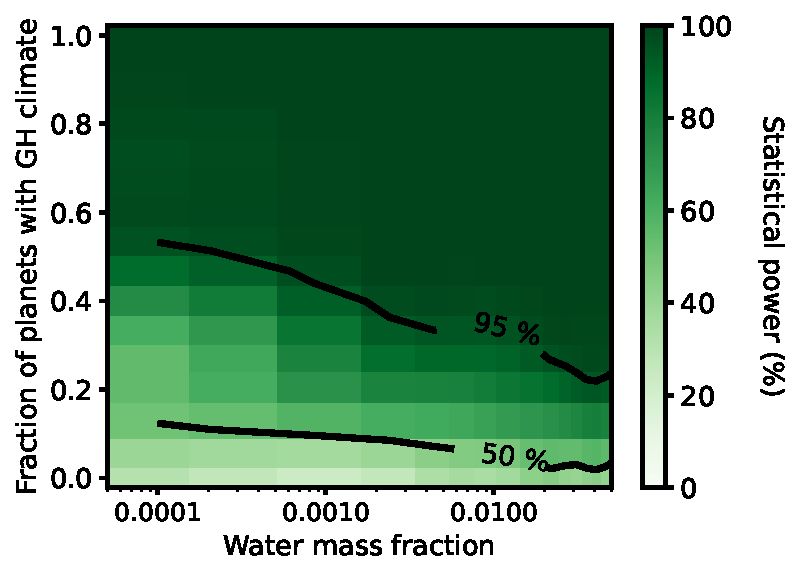
\includegraphics[width=\linewidth]{figures/optimistic_statpwr_H2O-f.pdf}
        \caption{
            Statistical power of the runaway greenhouse hypothesis test as a function of model parameters.
            For a sample size $N = \var{N_optimistic}$, the color code shows the fraction of simulations resulting in a sound detection ($\Delta \ln \mathcal{Z} > 3$) for different combinations of water mass fraction and fraction of greenhouse climate planets.
            Higher values in either parameter result in a more reliable detection.
            For water mass fractions $\gtrsim 10^{-4}$, the statistical power largely depends on the fraction of greenhouse climate planets in the sample.
        }
        \label{fig:statpwr_H2O-f}
    \end{centering}
\end{figure}
Figure~\ref{fig:statpwr_H2O-f} explores the statistical power achieved in the above scenario for different combinations of the poorly constrained parameters $x_{H_2O}$ and $f_\mathrm{rgh}$.
The higher the water content and thus the radius change, and the higher the fraction of planets in runaway greenhouse climates, the greater the prospect of a statistically sound detection.
 For all but very low water fractions, $f_\mathrm{rgh}$ dominates this trend: It enters linearly into the average planet radius, whereas the contribution of $x_{H_2O}$ - as predicted by the geophysical models - is sublinear with a power-law exponent of $\sim 0.3$.
As long as $f_\mathrm{rgh}$ is larger than $\sim 0.2$, a sample size of \var{N_optimistic} is sufficient for a $\SI{50}{\percent}$ detection rate even for water ratios as low as $10^{-3}$.



\subsection{Detecting the runaway greenhouse transition with current and planned exoplanet missions}\label{sec:res_samplesize}
\todo{Introduce survey simulation(s). PLATO, Cheops, (Ariel, LIFE/LIFE precursor, Nautilus)\\ What are threshold missions that are able to detect this signal? =>X meter working for Y years, or X' meter working for Y' years => conclusion could be that there is interesting science to do with intermediate size telescope.}
Under real-world conditions, the planetary properties in question can only be probed with a finite precision that is specific to each exoplanet mission.
%\subsubsection{PLATO}
\plato\ (PLAnetary Transits and Oscillation of stars) is an ESA mission designed to characterize terrestrial planets in the habitable zones of Sun-like stars, a goal to be achieved via long-term high-precision photometric monitoring of a sample of bright stars~\citep{Rauer2016}.
The \plato\ team has released an estimate on the number of exoplanets that will be characterized in the course of the main survey mission (Matuszewski, priv. comm.).
In the FGK sample of the mission, several hundred Earth-sized (\SIrange{0.8}{1.25}{\rEarth}) planets are expected to be detected.
\plato's definition study report~\citep{plato2017} further states precision requirements for planet radii~(\SI{3}{\percent}), planet masses through radial velocity follow-up~(\SI{10}{\percent}), and stellar masses, radii, and ages~(\SI{10}{\percent}).
We base our assessment of \plato's diagnostic power on these estimates.

    \begin{figure*}[ht!]
%    \script{figurescript.py}
        \begin{centering}
            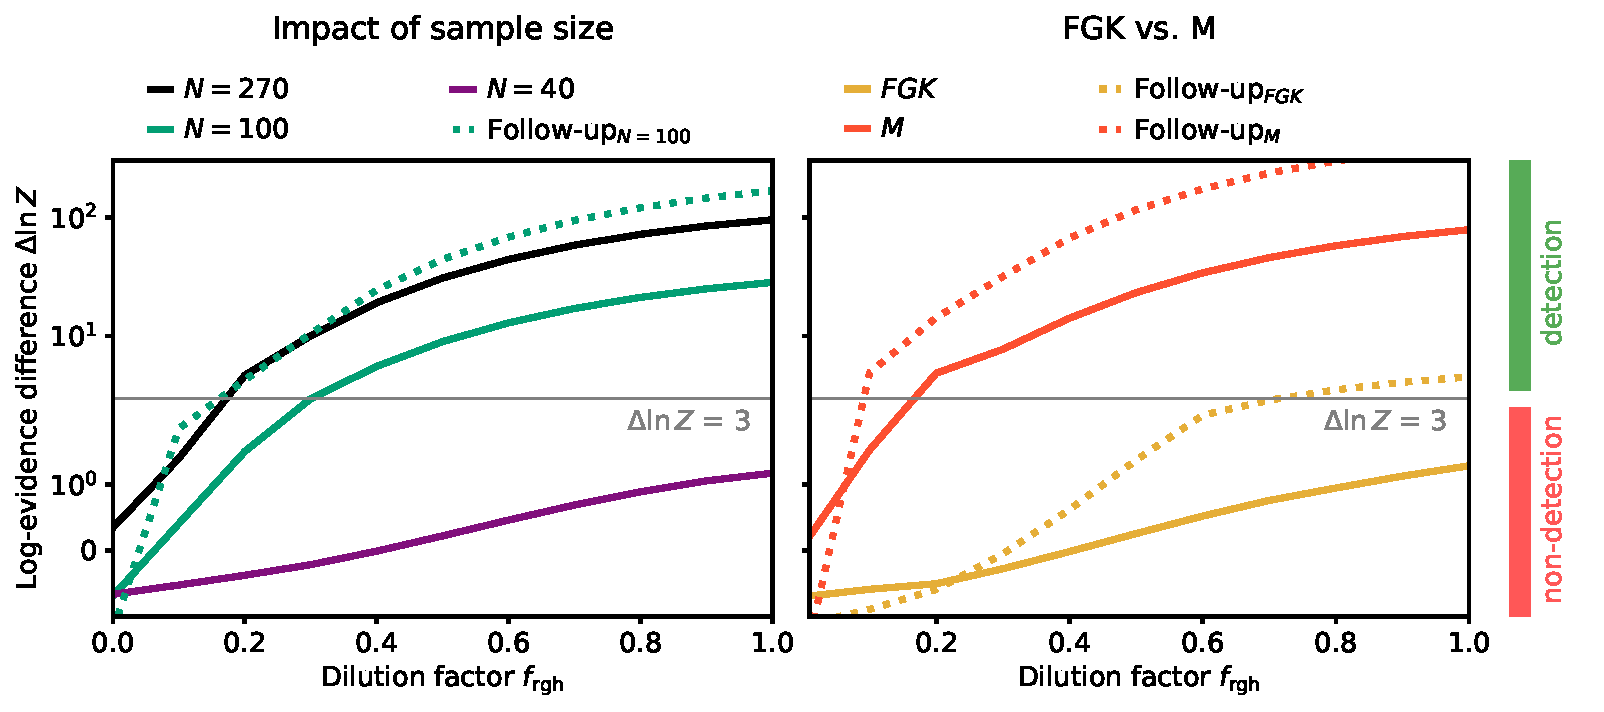
\includegraphics[width=\linewidth]{figures/plato_fgrid.pdf}
            \caption{
            Expected delta-evidences as a function of the fraction of planets harboring runaway greenhouse climates for different versions of the \plato\ survey.
            Median and $[16\mathrm{th}, 84\mathrm{th}]$ percentiles of randomized survey simulations are shown; $\Delta \ln Z > 3$ (gray horizontal line) is considered sufficient evidence to reject the null hypothesis.
            \textit{Left:} For a large planet yield of $N = \var{N_plato}$, even small planet fractions $\sim \var{platoMinfrgh}$ allow a detection.
                A sample of 100 planets is sufficient if their masses are constrained to within \SI{10}{\percent} (dotted green line).
                Without such follow-up measurements, sufficient diagnostic power can only be achieved with this sample if $f_\mathrm{rgh} \gtrsim \var{platoMinfrghHundred}$.
               Even smaller samples are unlikely to yield a significant detection.
            \textit{Right:} Evidences when only FGK or only M~dwarfs are considered.
                Only M~dwarfs host enough planets on both sides of the threshold instellation to allow a reliable detection of the runaway greenhouse signal.
            }
            \label{fig:plato_fgrid}
        \end{centering}
    \end{figure*}

For a volume-limited sample, considering all host star spectral types, we find that a yield of \var{N_plato} planets enables a significant detection if the fraction of runaway greenhouse planets is larger than $\sim \var{platoMinfrgh}$ (see Fig.~\ref{fig:plato_fgrid}).
The minimum needed fraction rises to \var{platoMinfrghHundred} for $N = 100$.
For much smaller samples, even an optimistically strong signal can no longer be detected.

What other planned missions are suited to test the runaway greenhouse hypothesis?
The ongoing \cheops\ mission was designed as a follow-up mission to search for transits of planets discovered with other techniques, in particular with radial velocity measurements~\citep{Benz2021}.
As such, it will provide precise radius constraints on a sample of small planets; however, only a small number of planets with periods \SI{> 50}{\day} are being observed.
This largely limits \cheops' coverage to planets within the runaway greenhouse regime, preventing a detection of the transition.

As \cheops, \ariel~\citep{Puig2016} will be a follow-up mission that is not designed to provide a large number of new radius measurements.
\ariel's primary targets are larger planets in the range of sub-Neptune to Jupiter-like planets.
We thus do not expect a significant contribution to exploring the inner edge of the habitable zone for Earth-sized planets.


\subsection{Statistical power of different mission designs}\label{sec:statpower_missions}
To explore the impact of mission trade-offs on the detectability of the runaway greenhouse transition, we simulated several transit surveys with different designs and strategies and measured their capability to recover the trend and constrain its parameters.
We assessed this capability based on two determinants: the likelihood that the mission is able to detect the injected trend, and the precision with which it can constrain the parameters of that trend.

\subsubsection{Additional planet mass measurements}
The dependencies of a detection change when additional information beyond planet radii is available for the characterized planet population.
Since the planet bulk density $\rho \propto R^{-3}$, the signal is stronger when measured in bulk density instead of radius:
With an optimistic choice of geophysical parameters (see above), the average measured radius change is \SI{+15}{\percent} whereas the average density change is \SI{-33}{\percent}.
Constraining bulk densities requires planetary mass measurements.
We now examine the value of a follow-up campaign to constrain planet masses with respect to the detectability of the runaway greenhouse threshold.

For uncertainties in density measurements, we propagate normally distributed errors of mass measurements assuming $\sigma_\mathrm{M_\mathrm{P}} = \SI{10}{\percent}$, as expected for \plato.
As can be seen in Fig.~\ref{fig:plato_fgrid}, the detectability is enhanced when radius constraints can be augmented with mass measurements: At unchanged sample size, the difference in Bayesian evidence can be up to an order of magnitude larger.
Consequently, we achieve a statistically significant detection with smaller samples or lower fractions $f_\mathrm{rgh}$.
A density-based survey of 100 targets is roughly equivalent to a radius-based survey of \var{N_plato} targets.
At $N=100$, pure radius measurements require $f_\mathrm{rgh} \gtrsim 0.4$ whereas bulk density measurements enable a detection from $f_\mathrm{rgh} \gtrsim 0.1$.

\subsubsection{Spectral type of target stars}\label{sec:results_FGK_M}
Since receiving radiation is sensitive on the spectral type of the host star, the share of planets on either side of $S_\mathrm{thresh}$ is different for FGK and M~dwarfs.
We tested the detectability of the runaway greenhouse signal when only FGK or only M~dwarfs are considered (see Fig.~\ref{fig:plato_fgrid}).
%($d_\mathrm{max} = \SI{75}{\parsec}, M_\mathrm{G} < 11$)
The samples are volume and magnitude-limited to reflect the target counts of \plato's provisional Long-duration Observation Phase fields~\citep[$15996$ FGK stars in the P1 and P2 samples, $33948$ M~stars in the P4 sample, ][]{Nascimbeni2022}.
The resulting M~dwarf planet sample is significantly larger with $\var{N_M}\pm \var{N_M_err}$ planets compared to $\var{N_FGK}\pm \var{N_FGK_err}$ planets in the FGK sample.
No significant detection is possible in the pure FGK sample, independent of the assumed geophysical parameters.
In the M~dwarf sample, the evidence threshold is reached around $f_\mathrm{rgh} \sim 0.2$, similar to the case above where all spectral types are considered.


\subsubsection{Constraining the threshold instellation}
\begin{figure}[ht!]
%    \script{figurescript.py}
    \begin{centering}

        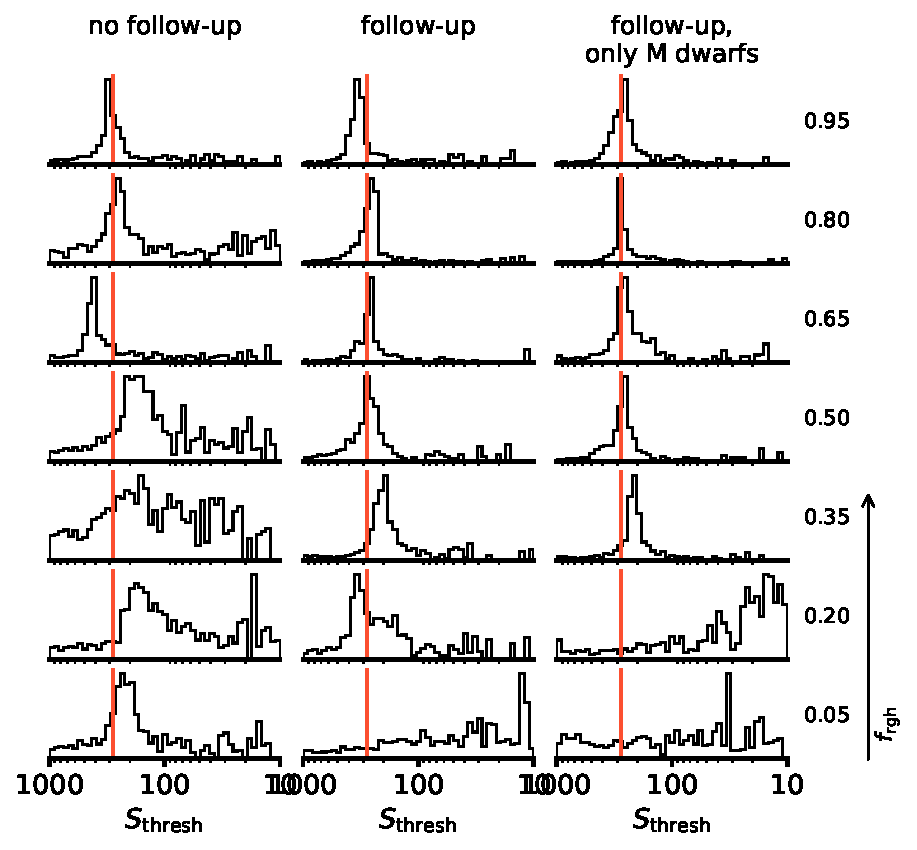
\includegraphics[width=\linewidth]{figures/S_thresh_posteriors.pdf}
        \caption{
            Retrieved posterior distributions of the threshold instellation for different survey realizations.
            All cases assume $x_{H_2O}$ and a planet sample size $N=100\pm10$; The fraction of planets with runaway greenhouse climates varies across rows.
            Orange lines show the true value of the injected signal.
            Accuracy and precision of the constraint on $S_\mathrm{thresh}$ generally improve with higher $f_\mathrm{rgh}$.
            Bulk density-based inferences improve the constraints.
        }
        \label{fig:posterior_surveys}
    \end{centering}
\end{figure}
A key constraint resulting from a successful detection is a measurement of $S_{thresh}$.
Here, we assess the ability of different mission concepts explored above to constrain this parameter.
Figure~\ref{fig:posterior_surveys} shows posterior distributions from a grid of inferences together with the true values of the injected signal for different fractions $f_\mathrm{rgh}$.
We consider three cases: only radius measurements, radius and mass measurements, and radius and mass measurements of only planets orbiting M~dwarfs.
The simulations otherwise represent the simulated PLATO example described above.
We chose a planetary sample size of $N=100\pm10$, as this was found to be a threshold case in Sect.~\ref{sec:res_samplesize}.

Accurate retrievals from radius measurements alone require high fractions of greenhouse climate-bearing planets to achieve an accurate constraint on $S_\mathrm{thresh}$.
If, on the other hand, a follow-up campaign adds planetary mass estimates and we fit the signal in bulk density space, useful constraints are possible under more pessimistic conditions.
A sample containing only planets around M~dwarf yields a comparable performance as the overall sample.


% Additional \subsection for habitability? To reflect structure in Discussion, Conclusions?

\section{Discussion}\label{sec:discussion}
\todo[inline]{\textbf{Potential discussion points: } what is the fraction of \kepler\ planets w/ runaway GH.}

\subsection{Statistical imprint of exoplanet climates}
\todo[inline]{the predicted climate tipping point causes a demographic imprint.\\
Discuss our ignorance on $f_\mathrm{rgh}$ and its impact on the imprint.}

\subsection{Detectability of the runaway greenhouse threshold}
\todo[inline]{the demographic imprint is detectable. Under what conditions?\\
Mention multiplanet systems.}

%We consider a number of key parameters of transit surveys: The telescope's mirror diameter (or effective diameter for a telescope array) $D$, the total time budget of the survey for observations $t_\mathrm{total}$, the maximum number of observed transits for each target $N_\mathrm{obs, max}$, the slew time between observations $t_\mathrm{slew}$, ... \todo[]{double-check which survey params are needed}
We identified the following drivers of the diagnostic power for detecting the runaway greenhouse transition with a given transit survey:
\begin{itemize}
    \item Prevalent water inventory: The magnitude of radius change at the runaway greenhouse threshold is highly sensitive on water mass fraction. As a result, the statistical abundance of water in terrestrial planets impacts the strength of the demographic pattern.
    \item Sample size: Since we are looking for a population-level trend, the statistical significance will increase with a larger sample size.
    \item Radius measurement precision: The more precise individual planet radii can be determined, the less smeared out the pattern will be. Good \textit{accuracy} is less important, as long as it does not have a systematic error scaling with stellar irradiance.
    \item Availability and precision of mass measurements: For simple geometric reasons ($\rho \propto R^{-3}$), the expected trend is stronger when measured in bulk density than it is in planet radius space. If transiting planets can be followed up to obtain mass measurements, the statistical significance increases.
\end{itemize}
Besides these main factors, uncertainties in the measured instellations can influence the result, although they are typically small due to the very precise orbital period measurements available for transiting planets.
This can be different for young host stars when their ages can not be well constrained; in particular the long pre-main sequence phase of M~dwarfs shows a large variation in bolometric luminosity~(see Fig.~\ref{fig:luminosity_tracks}).



\subsubsection{False positive scenarios}
\todo{what other processes could be confused with a magma ocean signal?}
\begin{note}
    Global magma oceans are not the only physical mechanism that may cause a decrease in transit radii for a subset of planets.
    Other causes of shrinking planet sizes have been put forward, the most widely discussed ones being atmospheric loss due to either photoevaporation through high-energy radiation by the host star~\citep[e.g.,][]{Owen2013,Jin2014,Mordasini2020a} or due to residual heat from the planet's interior shortly after formation~\citep{Ginzburg2016b,Ginzburg2018,Gupta2019}.
    Both processes are being traded as potentially sculpting the observed radius bimodality of small, close-in exoplanets from the  mission~\citep{Fulton2017,VanEylen2018}.
    Like the magma ocean effect discussed here, these processes reduce the radii of some planets, leading to a decrease in average measured planet radii in a specific region of the planetary parameter space.
    This region is distinct from the one affected by global magma oceans, since... \todo{...elaborate why they cannot be confused}

    Another false positive contribution may come from potential unknown variations in the occurrence rate gradients in radius-instellation space.
    They can impact the statistical inference of the transitions, especially if these variations are similar to the expected pattern.
    Although an abrupt pattern at the expected runaway greenhouse transition seems unlikely, examples of steep occurrence rate density changes exist.
    An example is the "Neptune desert``, a triangular region of low planet occurrence density of close-in planets in period-radius space~\citep{Szabo2011,Mazeh2016,Dreizler2020b}.
    The shape of this region is such that smaller planets become less frequent the closer to the star they are, which to some degree resembles the pattern introduced by the instellation dependency of the magma ocean probability.
    However, the Neptune desert occurs at smaller orbital periods and its location depends on a planet's size~\citep{Szabo2011}, which is not expected for the runaway greenhouse transition.
    \todo{is there overlap/confusion with the radius/density trend in \citet{Luque2022b}?}
\end{note}

%\todo[inline]{Maps to Sect. \ref{sec:statpower_missions}.:}
%\begin{note}
%    \citet{Penny2019} mention that a significant increase in planet yield could be achieved if the telescope's slew speed was increased.
%\end{note}



\subsubsection{OPTIONAL...: Atmospheric signatures}
\todo[inline]{discuss potential atmospheric signatures of magma oceans. e.g.: H/O ratios of sub-Neptunes could be low (because H is in the melt) (Tim's talk)}


\subsection{Diagnostic power of upcoming exoplanet missions}\todo[inline]{\plato: needed sample size, precision}
The fidelity of a future detection or falsification of a magma ocean signature will depend on the significance with which the null hypothesis can be excluded.
As a consequence, instrumentation and survey strategy aiming at testing the hypothesis should aim at maximizing the probability of a true positive detection given the existence of the effect.
...

\subsection{Mission design trades}\label{sec:mission-design-trades}
We now turn to mission design trades that influence the statistical power for testing the runaway greenhouse hypothesis.
...
\subsubsection{The value of follow-up campaigns}
\begin{note}
...FOLLOW-UP...radial velocity follow-up measurements...

The advantage of mass measurements for the planet sample can be enhanced with a wise selection of follow-up targets, i.e. favoring those planets residing close to $S_\mathrm{thresh}$.
\end{note}

\subsubsection{Target star spectral types}
\begin{note}
    ...FGK vs. M...:

To date, the majority of planets with radius measurements orbit FGK~dwarfs and lie in the runaway greenhouse regime.
    ...

    Our tests with different spectral types (Sect.~\ref{sec:results_FGK_M}) show that the information content of M~dwarfs in a sample dominates the hypothesis tests.
The reason is, besides their large number in a volume/magnitude-limited sample, that many detected M~dwarf planets are located near the threshold instellation.
As in the cases above, an M~dwarf survey profits from follow-up measurements of planetary masses with an order of magnitude increase in evidence.

    An additional advantage of targeting M~dwarfs are their extended runaway greenhouse phases, whose duration can reach the order of \SI{100}{\mega\year}~CITE.
    This increases the probability of observing any given planet in the sample during the runaway greenhouse phase, essentially driving $f_\mathrm{rgh}$ to higher values.
\end{note}

\subsection{Implications for planetary habitability}\label{sec:habitability}
\todo[inline]{Magma oceans influence the amount of water available at the surface and atmosphere, which is 1. commonly used as environmental marker to assess habitability, and 2. influences the planet's climate (greenhouse effect).}



\section{Conclusions}
% Planetary radius changes due to the combined effect of steam atmospheres and water dissolved in the molten mantle of planets within the runaway greenhouse threshold is expected to cause a discontinuity in the radius distribution of small (DEFINITION) exoplanets.
Runaway greenhouse climates on Earth-like planets are thought to cause significant inflation of their radii.
Using Bioverse, a quantitative hypothesis testing framework, we have explored the potential of contemporary exoplanet missions to statistically detect a radius discontinuity resulting from this inflation in the exoplanet population.
Our key findings are as follows:
\begin{enumerate}
    \item The predicted tipping point in planetary climates causes a discontinuity in the radius and density distribution of small exoplanets with respect to the incident host star irradiation.
    \item The demographic imprint of the runaway greenhouse threshold should be detectable with high-precision transit measurements. For a large sample $\gtrsim 100$, a detection is likely if radius inflation occurs on at least \SI{10}{\percent} of planets and if typical water mass fractions are above $\sim 10^{-3}$.
    \item We find that the planned \plato\ transit survey will provide a sufficient sample and the required precision to detect the predicted trend. Assuming the projected photometric precision, \plato\ will be able to test the runaway greenhouse hypothesis for planet yields $\gtrsim 100$.
    \item The diagnostic power of transit missions in testing this hypothesis can be increased through a follow-up campaign providing planet mass measurements. This can reduce the required planet yield by up to a factor of five. An optimized survey will further focus on M~dwarfs to ensure sufficient targets on both sides of the expected threshold instellation.
    \item A detection of the feature will constrain the water inventory of rocky exoplanets, providing important context in the assessment of their habitability.
\end{enumerate}


%\begin{acknowledgments}
%The authors thank Yann Fabel, Paul Molliere, Matthew Murphy, and Terry-Ann Suer for insightful discussions.
%We are grateful to Martin Turbet for providing the mass-radius relationship data for planets harboring steam atmospheres.
%\end{acknowledgements}

\begin{large}\textit{Author contributions:}\end{large}

\section*{Data Availability}
All data sets and software required to reproduce our results and this article are available through GitHub and Zenodo.
The code to reproduce the figures can be accessed via the icon links associated with the respective figure caption.


\software{
Bioverse~\citep{Bixel2021},
Astropy~\citep[][]{AstropyCollaboration2018},
NumPy~\citep[][]{Harris2020},
SciPy~\citep[][]{Virtanen2020},
corner.py~\citep{Foreman-Mackey2016b},
dynesty~\citep{Speagle2020}.
}


\bibliographystyle{aasjournal}
\bibliography{bib,PhD}
\end{document}
